\documentclass[tikz,border=3pt]{standalone}
\usepackage{amsmath}
\usetikzlibrary{arrows.meta,positioning,fit,calc}
\definecolor{navy}{HTML}{153B5B}
\definecolor{blue}{HTML}{2D6A9F}
\definecolor{teal}{HTML}{2A9D8F}
\definecolor{gold}{HTML}{E9A23B}
\definecolor{red}{HTML}{C75C5C}
\definecolor{ink}{HTML}{24313A}
\definecolor{pale}{HTML}{F4F7F9}
\tikzset{
  box/.style={draw=navy, line width=.8pt, rounded corners=2pt,
    fill=pale, minimum height=9mm, align=center, font=\sffamily\small,
    inner xsep=4pt},
  branch/.style={box, minimum width=26mm},
  arrow/.style={-{Latex[length=2.2mm]}, line width=.8pt, draw=ink},
  note/.style={font=\sffamily\scriptsize, text=ink, align=center}
}
\begin{document}
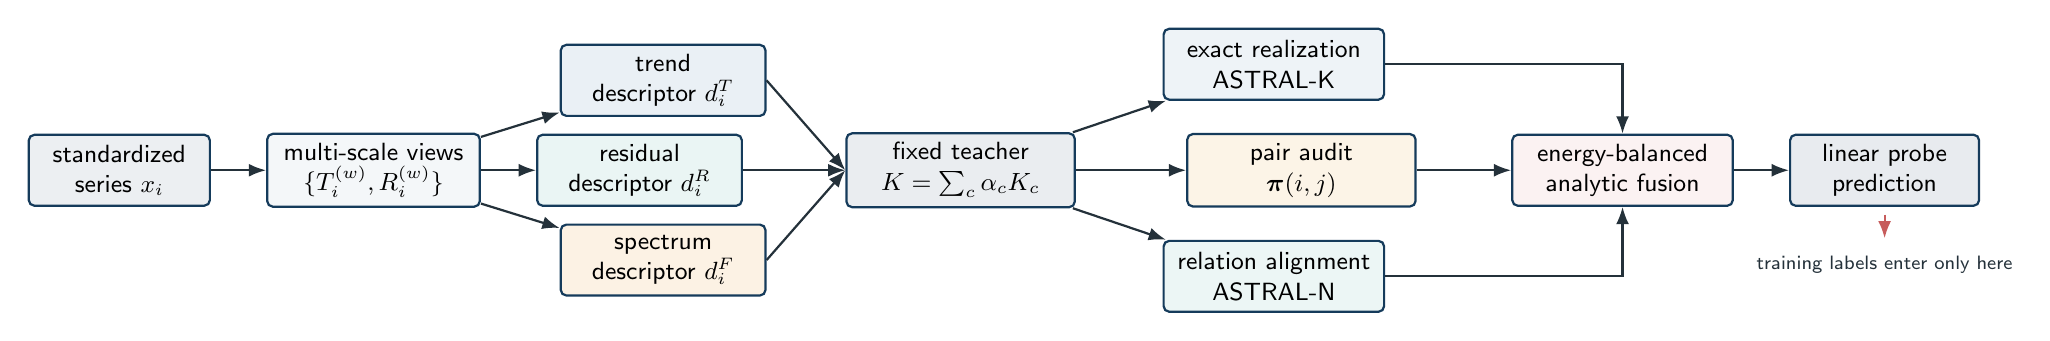
\begin{tikzpicture}[node distance=5mm and 7mm]
  \node[box,fill=navy!8,minimum width=23mm] (x) {standardized\\series $x_i$};
  \node[box,right=of x,minimum width=27mm] (views) {multi-scale views\\$\{T_i^{(w)},R_i^{(w)}\}$};

  \node[branch,above right=2mm and 10mm of views,fill=blue!10] (t) {trend\\descriptor $d_i^T$};
  \node[branch,right=of views,fill=teal!10] (r) {residual\\descriptor $d_i^R$};
  \node[branch,below right=2mm and 10mm of views,fill=gold!14] (f) {spectrum\\descriptor $d_i^F$};

  \node[box,right=13mm of r,minimum width=29mm,fill=navy!9] (teacher)
    {fixed teacher\\$K=\sum_c\alpha_cK_c$};
  \node[box,above right=4mm and 11mm of teacher,minimum width=28mm,fill=blue!8] (kpca)
    {exact realization\\ASTRAL-K};
  \node[box,below right=4mm and 11mm of teacher,minimum width=28mm,fill=teal!9] (neural)
    {relation alignment\\ASTRAL-N};
  \node[box,right=14mm of teacher,minimum width=29mm,fill=gold!12] (audit)
    {pair audit\\$\boldsymbol\pi(i,j)$};

  \node[box,right=12mm of audit,minimum width=28mm,fill=red!8] (fusion)
    {energy-balanced\\analytic fusion};
  \node[box,right=of fusion,minimum width=24mm,fill=navy!10] (probe)
    {linear probe\\prediction};

  \draw[arrow] (x) -- (views);
  \draw[arrow] (views) -- (t);
  \draw[arrow] (views) -- (r);
  \draw[arrow] (views) -- (f);
  \draw[arrow] (t.east) -- (teacher.west);
  \draw[arrow] (r.east) -- (teacher.west);
  \draw[arrow] (f.east) -- (teacher.west);
  \draw[arrow] (teacher) -- (kpca);
  \draw[arrow] (teacher) -- (neural);
  \draw[arrow] (teacher) -- (audit);
  \draw[arrow] (kpca.east) -| (fusion.north);
  \draw[arrow] (neural.east) -| (fusion.south);
  \draw[arrow] (audit) -- (fusion);
  \draw[arrow] (fusion) -- (probe);

  \node[note,below=5mm of probe] {training labels enter only here};
  \draw[arrow,draw=red] ([yshift=-1mm]probe.south) -- ++(0,-3mm);
\end{tikzpicture}
\end{document}
